%%%%%%%%%%%%%%%%%%%%%%%%%%%%%%%%%%%%%%%%%
% Short Sectioned Assignment
% LaTeX Template
% Version 1.0 (5/5/12)
%
% This template has been downloaded from:
% http://www.LaTeXTemplates.com
%
% Original author:
% Frits Wenneker (http://www.howtotex.com)
%
% License:
% CC BY-NC-SA 3.0 (http://creativecommons.org/licenses/by-nc-sa/3.0/)
%
%%%%%%%%%%%%%%%%%%%%%%%%%%%%%%%%%%%%%%%%%

%----------------------------------------------------------------------------------------
%	PACKAGES AND OTHER DOCUMENT CONFIGURATIONS
%----------------------------------------------------------------------------------------

\documentclass[paper=a4, fontsize=11pt]{scrartcl} % A4 paper and 11pt font size

\usepackage[T1]{fontenc} % Use 8-bit encoding that has 256 glyphs
\usepackage{fourier} % Use the Adobe Utopia font for the document - comment this line to return to the LaTeX default
\usepackage[english]{babel} % English language/hyphenation
\usepackage{amsmath,amsfonts,amsthm} % Math packages
\usepackage[utf8]{inputenc}
\usepackage{lipsum} % Used for inserting dummy 'Lorem ipsum' text into the template
\usepackage{xcolor}
\usepackage{graphicx}


\usepackage{listings}
  \usepackage{courier}
 \lstset{
         basicstyle=\footnotesize\ttfamily, % Standardschrift
         %numbers=left,               % Ort der Zeilennummern
         numberstyle=\tiny,          % Stil der Zeilennummern
         %stepnumber=2,               % Abstand zwischen den Zeilennummern
         numbersep=5pt,              % Abstand der Nummern zum Text
         tabsize=2,                  % Groesse von Tabs
         extendedchars=true,         %
         breaklines=true,            % Zeilen werden Umgebrochen
         keywordstyle=\color{red},
    		frame=b,         
 %        keywordstyle=[1]\textbf,    % Stil der Keywords
 %        keywordstyle=[2]\textbf,    %
 %        keywordstyle=[3]\textbf,    %
 %        keywordstyle=[4]\textbf,   \sqrt{\sqrt{}} %
         stringstyle=\color{white}\ttfamily, % Farbe der String
         showspaces=false,           % Leerzeichen anzeigen ?
         showtabs=false,             % Tabs anzeigen ?
         xleftmargin=17pt,
         framexleftmargin=17pt,
         framexrightmargin=5pt,
         framexbottommargin=4pt,
         %backgroundcolor=\color{lightgray},
         showstringspaces=false      % Leerzeichen in Strings anzeigen ?        
 }
 \lstloadlanguages{% Check Dokumentation for further languages ...
         %[Visual]Basic
         %Pascal
         %C
         %C++
         %XML
         %HTML
         Java
 }
    %\DeclareCaptionFont{blue}{\color{blue}} 

  %\captionsetup[lstlisting]{singlelinecheck=false, labelfont={blue}, textfont={blue}}
  \usepackage{caption}
\DeclareCaptionFont{white}{\color{white}}
\DeclareCaptionFormat{listing}{\colorbox[cmyk]{0.43, 0.35, 0.35,0.01}{\parbox{\textwidth}{\hspace{15pt}#1#2#3}}}
\captionsetup[lstlisting]{format=listing,labelfont=white,textfont=white, singlelinecheck=false, margin=0pt, font={bf,footnotesize}}


\usepackage{sectsty} % Allows customizing section commands
\allsectionsfont{\centering \normalfont\scshape} % Make all sections centered, the default font and small caps

\usepackage{fancyhdr} % Custom headers and footers
\pagestyle{fancyplain} % Makes all pages in the document conform to the custom headers and footers
\fancyhead{} % No page header - if you want one, create it in the same way as the footers below
\fancyfoot[L]{} % Empty left footer
\fancyfoot[C]{} % Empty center footer
\fancyfoot[R]{\thepage} % Page numbering for right footer
\renewcommand{\headrulewidth}{0pt} % Remove header underlines
\renewcommand{\footrulewidth}{0pt} % Remove footer underlines
\setlength{\headheight}{13.6pt} % Customize the height of the header

\numberwithin{equation}{section} % Number equations within sections (i.e. 1.1, 1.2, 2.1, 2.2 instead of 1, 2, 3, 4)
\numberwithin{figure}{section} % Number figures within sections (i.e. 1.1, 1.2, 2.1, 2.2 instead of 1, 2, 3, 4)
\numberwithin{table}{section} % Number tables within sections (i.e. 1.1, 1.2, 2.1, 2.2 instead of 1, 2, 3, 4)

\setlength\parindent{0pt} % Removes all indentation from paragraphs - comment this line for an assignment with lots of text

%----------------------------------------------------------------------------------------
%	TITLE SECTION
%----------------------------------------------------------------------------------------

\newcommand{\horrule}[1]{\rule{\linewidth}{#1}} % Create horizontal rule command with 1 argument of height

\title{	
\normalfont \normalsize 
\textsc{ENSEIRB-MATMECA} \\ [25pt] % Your university, school and/or department name(s)
\horrule{0.5pt} \\[0.4cm] % Thin top horizontal rule
\huge Accélérateurs de calculs \\ % The assignment title
\horrule{2pt} \\[0.5cm] % Thick bottom horizontal rule
}

\author{Caneill Pierre-Yves, Lux Benjamin} % Your name

\date{\normalsize\today} % Today's date or a custom date

\begin{document}

\maketitle % Print the title

%----------------------------------------------------------------------------------------
%	Version 1
%----------------------------------------------------------------------------------------

\section{Multiplication de matrices}
Nous avons réalisé cette partie en \verb!CUDA!.
\subsection{Version Simple}
Le premier kernel est très simple, chaque thread de calcul va se
charger de calculer sa case de la matrice.

Bien que cette version soit très simple on arrive à obtenir des
résultats bien plus interessant que sur CPU.

\subsection{Optimisation mémoire}
La deuxième version va esseyer d'optimiser les accès mémoire en
travaillant par rangée. Ainsi les différents wrap accèderont à des
données proches.

\subsection{Optimisation par blocs}
Enfin la dernière optimisation que nous avons fait était de faire des
calculs matriciels par blocs. Afin de réutiliser la mémoire. Pour cela
nous avons chargé en mémoire partagée le bloc de travail pour ensuite
faire les calculs.

\begin{lstlisting}
__global__ void matrixMul3(float * g_C, float * g_A, float *g_B,int wa, int wb){
  const int TILE_WIDTH = 16;
  int tx = threadIdx.x;
  int ty = threadIdx.y;
  int bx = blockIdx.x;
  int by = blockIdx.y;

  __shared__ float s_a[TILE_WIDTH][TILE_WIDTH];
  __shared__ float s_b[TILE_WIDTH][TILE_WIDTH];

  int row = bx*blockDim.y + tx;
  int col = by*blockDim.x + ty;
  float result = 0;

  int i = 0;
  for(i = 0; i < wa/TILE_WIDTH; ++i){
    s_a[tx][ty] = g_A[i*TILE_WIDTH + row*wa +ty];
    s_b[tx][ty] = g_B[(i*TILE_WIDTH*wa)+tx*wa+ col];
    __syncthreads();

    int k =0;
    for(k=0;k<TILE_WIDTH;++k){
      result += s_a[tx][k] * s_b[k][ty];
    }
    __syncthreads();
  }

  g_C[row*wa+col] = result;

}
\end{lstlisting}


\subsection{Comparaison des différentes versions}
Nous avons implémenté une version sur le processeur en utilisant
openMP.

Le premier graphique présente les différentes version GPU avec la
version CPU. On observe que la version CPU prend énormément plus de
temps que les différentes version GPU.
\begin{figure}[!h]
  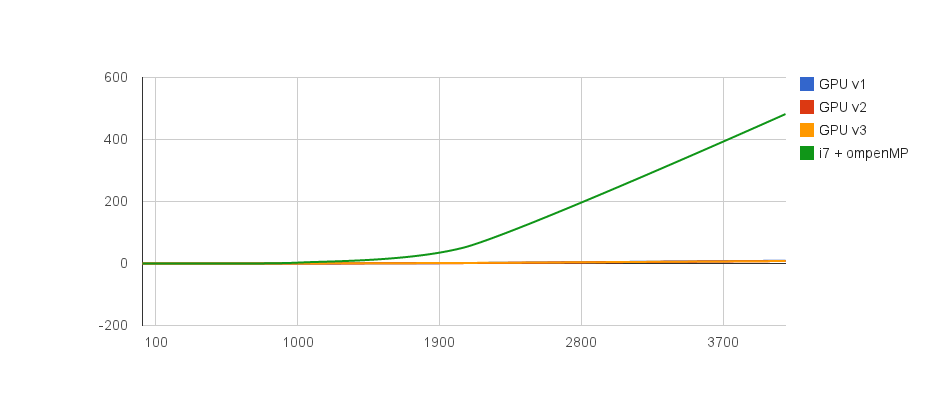
\includegraphics[width=1\textwidth]{chart_1.png}
  \centering
  \caption{Comparaison GPU / CPU}
\end{figure}

Le deuxième graphique présente une comparaison des différentes
versions GPU entre elles. On voit que elles sont dans le même ordre de
grandeur. On a été assez surpris que la version par blocs n'aille pas
significativement plus vite que les autres. S'est peut être lié à une
erreur d'implémentation.

\begin{figure}[!h]
  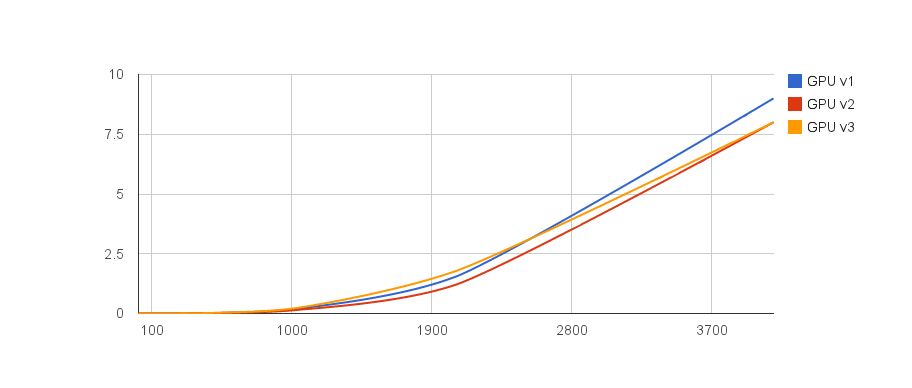
\includegraphics[width=1\textwidth]{chart_2.png}
  \centering
  \caption{Comparaison GPU}
\end{figure}

\subsection{Sortie du programme}
\begin{verbatim}
System Informations
-------------------

Number of devices : 1
Device Informations
  Name : GeForce GT 555M
  Memory : 2147155968
  WarpSize : 32
  Max Threads Per Block : 1024
  Multi processor count : 3


Multiplication with CPU using openMP
-----------------------------------

Size Matrix 2048x2048
Starting multiplication CPU ...[OK]
Time : 47.579655 s
Mflop/s : 361.075951 


Multiplication without optimisation
-----------------------------------

Size Matrix 2048x2048

Starting multiplication GPU ...[OK]
Time : 1.525846 s
Mflop/s : 11259.256637 
Multiplication correct
Speed UP x30


Multiplication with first optimisation
-----------------------------------------

Size Matrix 2048x2048
Starting multiplication GPU ...[OK]
Time : 1.198078 s
Mflop/s : 14339.536761 
Multiplication correct
Speed UP x39


Multiplication with second optimisation
-----------------------------------------

Size Matrix 2048x2048
Starting multiplication GPU ...[OK]
Time : 1.761853 s
Multiplication correct
Speed UP x26
\end{verbatim}



\section{Factorisation de Cholesky}



\end{document}



